\section{Resultados}
\label{sec:resultados}

Todas las cifras de esta sección provienen de
\path{reports/final/resultados.csv}, que el notebook de la
Sección~\ref{sec:repo} reconstruye a partir de los \texttt{history.csv} y
\texttt{eval\_report.json} de cada corrida. Salvo que se indique otra cosa,
las métricas son de validación (3,712 imágenes) en el checkpoint con mayor F1
macro.

\subsection{Desbalance de clases}
\label{sec:desbalance}

El conjunto de entrenamiento tiene 12,753 imágenes repartidas de forma muy
desigual entre las 104 clases (Figura~\ref{fig:distribucion}). La clase más
pequeña tiene 18 imágenes (\emph{moon orchid}, \emph{bolero deep blue} y
\emph{alpine sea holly}) y la más grande 782 (\emph{iris}): una razón de
43:1. La mediana es de 88 imágenes y la media de 122.6; la media queda por
encima de la mediana porque unas pocas clases concentran los datos: las 10 más
grandes reúnen el 40\% de las imágenes, mientras que 24 clases tienen menos de
30. El rango intercuartílico va de 32.5 a 125.5 imágenes. Validación conserva
exactamente las mismas proporciones (de 5 a 228 imágenes por clase), de modo
que las clases raras tienen también muy pocos ejemplos para evaluarlas: el F1
de una clase con 5 imágenes de validación cambia en más de 0.15 con un solo
acierto.

\begin{figure*}[htbp]
\centering
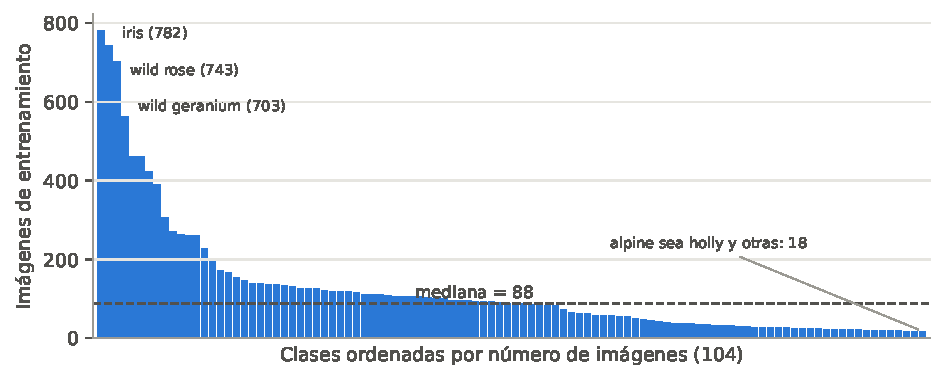
\includegraphics[width=0.85\textwidth]{distribucion_clases.pdf}
\caption{Imágenes de entrenamiento por clase, ordenadas de mayor a menor. La
línea punteada marca la mediana (88).}
\label{fig:distribucion}
\end{figure*}

\subsection{Arquitecturas: MLP, CNN de referencia y CNN ampliada}
\label{sec:res-arquitecturas}

La Tabla~\ref{tab:modelos} resume las arquitecturas y la
Figura~\ref{fig:curvas-modelos} muestra sus curvas de pérdida, exactitud y F1
macro en entrenamiento y validación. La CNN de referencia alcanza un F1 macro de
0.5784 y una exactitud de 64.06\%; la MLP, con 20 veces más parámetros, se
queda en 0.0178 y 14.36\%. La CNN ampliada llega a 0.5663, por debajo de la
referencia. Su corrida se interrumpió en la época 50 por un bloqueo de la GPU;
como su F1 de validación llevaba ocho épocas estable alrededor de 0.564 y la
tasa de aprendizaje ya había bajado a $3\times10^{-5}$, es poco probable que
hubiera alcanzado a la referencia.

\begin{table*}[htbp]
\centering
\caption{Arquitecturas comparadas con los mismos datos de validación (3,712 imágenes).}
\label{tab:modelos}
\small
\begin{tabular}{lrrrrrrr}
\toprule
Modelo & Parámetros & Época & Exact. (\%) & F1 entr. & Brecha F1 & Tiempo (min) & F1 macro \\
\midrule
MLP & 9,660,776 & 62/74 & 14.36 & 0.0192 & +0.0014 & 6.9 & 0.0178 \\
CNN de referencia & 480,936 & 91/103 & 64.06 & 0.8138 & +0.2354 & 19.7 & \textbf{0.5784} \\
CNN ampliada (6 conv.)$^\dagger$ & 1,218,600 & 41/49 & 63.77 & 0.7936 & +0.2273 & 17.1 & 0.5663 \\
\bottomrule
\end{tabular}
\par\smallskip
\parbox{0.95\textwidth}{\footnotesize Época: checkpoint elegido por F1 macro / épocas ejecutadas. F1 entr.: F1 macro sobre 3,712 imágenes fijas de entrenamiento sin aumento ni dropout, en la misma época. Brecha F1 = F1 entr. $-$ F1 macro de validación. Todas a 112$\times$112, entrenadas desde cero con semilla 0. $^\dagger$La corrida se interrumpió en la época 50 por un bloqueo de la GPU; se reporta su mejor checkpoint.}
\end{table*}


\begin{figure*}[htbp]
\centering
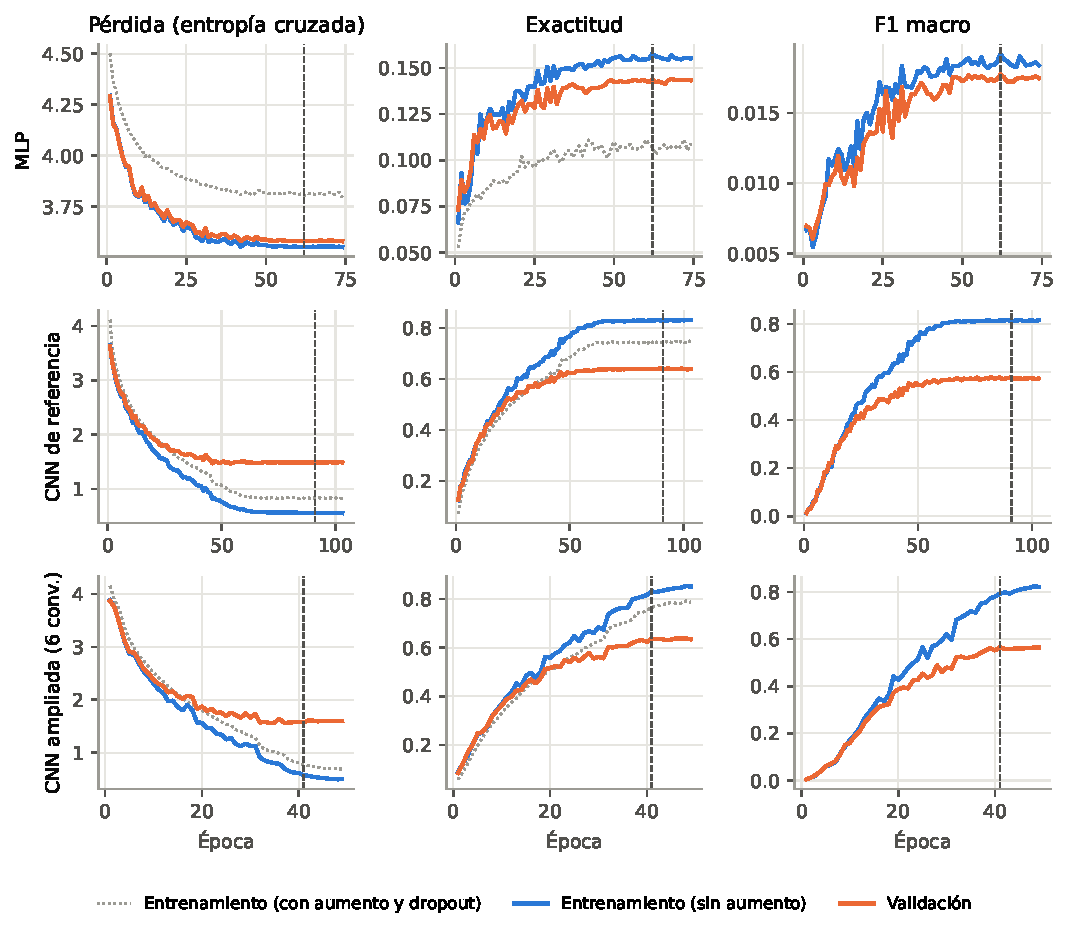
\includegraphics[width=\textwidth]{curvas_modelos.pdf}
\caption{Curvas de entrenamiento y validación por época. Azul: 3,712 imágenes
fijas de entrenamiento sin aumento, en modo inferencia. Naranja: validación.
Gris punteado: la métrica que reporta el ciclo de entrenamiento, con aumento y
dropout activos (no existe para el F1). La línea vertical marca el checkpoint
elegido. Las escalas verticales de la MLP son distintas.}
\label{fig:curvas-modelos}
\end{figure*}

Las curvas muestran tres comportamientos distintos:

\begin{itemize}
\item \textbf{CNN de referencia: sobreajuste moderado y controlado.} Las dos
curvas avanzan juntas durante unas 15 épocas y después se separan. La pérdida de
validación toca su mínimo en la época 54 (1.464) y después apenas sube (1.486 al
final), mientras el F1 de validación sigue mejorando poco a poco hasta
la época 91. En el checkpoint, el F1 de entrenamiento es 0.8138 y el de
validación 0.5784: una brecha de 0.235.
\item \textbf{CNN ampliada: el mismo techo, alcanzado antes.} Con 2.5 veces más
parámetros aprende el entrenamiento más rápido (en la época 41 su F1 de
entrenamiento es 0.794 frente a 0.638 de la referencia), pero su validación se
estanca en el mismo nivel. Su pérdida de validación toca su mínimo antes (época
34) y después sube de 1.555 a 1.602, una señal de sobreajuste más clara que en
la referencia.
\item \textbf{MLP: infraajuste.} Entrenamiento y validación casi coinciden
(brecha de F1 de 0.001) y ambas son muy bajas. La red no memoriza: no logra
aprender. Solo predice 11 de las 104 clases y tiene F1 = 0 en 93.
\end{itemize}

En las tres redes, la curva gris queda por debajo de la azul: el aumento de datos
y el dropout hacen que las métricas del ciclo de entrenamiento parezcan peores
de lo que el modelo realmente rinde sobre imágenes de entrenamiento.

La Tabla~\ref{tab:ultima-epoca} justifica conservar el checkpoint con mayor F1
macro y no la última época. Entre la época 91 y la 103, el modelo sigue
ajustando un poco el entrenamiento (la pérdida baja de 0.557 a 0.551), pero el
F1 de validación cae de 0.5784 a 0.5731 y su pérdida sube. La diferencia entre
exactitud (64.06\%) y F1 macro (0.578) también es informativa: la exactitud
cuenta aciertos sobre todas las imágenes y la dominan las clases grandes; el F1
macro promedia por clase, así que pesa igual una clase de 18 imágenes que
\emph{iris} con 782.

\begin{table}[htbp]
\centering
\caption{CNN de referencia en la época elegida y al terminar el entrenamiento.}
\label{tab:ultima-epoca}
\small
\begin{tabular}{lrr}
\toprule
Métrica & Elegida (91) & Última (103) \\
\midrule
\multicolumn{3}{l}{\textit{Entrenamiento}} \\
\quad Exactitud (\%) & 83.00 & 83.05 \\
\quad F1 macro & 0.8138 & 0.8145 \\
\quad Pérdida & 0.557 & 0.551 \\
\multicolumn{3}{l}{\textit{Validación}} \\
\quad Exactitud (\%) & 64.06 & 63.95 \\
\quad F1 macro & 0.5784 & 0.5731 \\
\quad Pérdida & 1.483 & 1.486 \\
\bottomrule
\end{tabular}
\par\smallskip
\parbox{0.95\columnwidth}{\footnotesize Entre paréntesis, la época. Entrenamiento: 3,712 imágenes fijas sin aumento, en modo inferencia.}
\end{table}


\subsection{Comparación con el Avance~4}

La Tabla~\ref{tab:avance4} contrasta estas corridas con las del Avance~4. El F1
de la referencia se reproduce (0.5745 frente a 0.5784) aunque cambió el
\emph{framework}, lo que da confianza en la comparación. Lo que cambia es la
brecha: medida con aumento y dropout activos, como en el Avance~4, la brecha de
exactitud de la referencia era de 0.105; medida sobre imágenes limpias es de
0.189 en exactitud y de 0.235 en F1 macro. El Avance~4 subestimaba el
sobreajuste a casi la mitad. En la CNN ampliada, que en el Avance~4 se entrenó
con Adam y tasa fija, la misma política de la referencia reduce su desventaja de
0.024 a 0.012 puntos de F1, pero no la elimina.

\begin{table*}[htbp]
\centering
\caption{Avance 4 frente al reporte final: la brecha medida con aumento subestima el sobreajuste.}
\label{tab:avance4}
\small
\begin{tabular}{llrrrrr}
\toprule
Modelo & Política en Avance 4 & F1 A4 & Brecha exact. A4 & F1 final & Brecha exact. & Brecha F1 \\
\midrule
CNN de referencia & AdamW + LR adaptable & 0.5745 & +0.1051 & 0.5784 & +0.1894 & +0.2354 \\
CNN ampliada (6 conv.) & Adam, LR fijo & 0.5502 & +0.1687 & 0.5663 & +0.1926 & +0.2273 \\
MLP & Adam, LR fijo & 0.0280 & -0.0346 & 0.0178 & +0.0140 & +0.0014 \\
\bottomrule
\end{tabular}
\par\smallskip
\parbox{0.95\textwidth}{\footnotesize A4: PyTorch/DirectML; su exactitud de entrenamiento se midió durante el ciclo, con aumento y dropout activos. Final: TensorFlow/Metal, todas con AdamW + LR adaptable; brechas medidas sobre 3,712 imágenes de entrenamiento sin aumento y en modo inferencia, en la época del checkpoint.}
\end{table*}


\subsection{F1 por clase de la CNN de referencia}
\label{sec:por-clase}

El F1 macro de 0.578 esconde mucha variación entre clases
(Tabla~\ref{tab:clases}). La mediana por clase es 0.600; 16 clases superan 0.8 y
13 quedan por debajo de 0.3. Las mejores son flores con forma o color muy
característicos (\emph{pink-yellow dahlia} y \emph{cautleya spicata} con F1 de
1.0, \emph{cape flower} y \emph{purple coneflower} con 0.97). Cinco clases tienen
F1 = 0: \emph{bolero deep blue}, \emph{siam tulip}, \emph{canterbury bells},
\emph{pink quill} y \emph{garden phlox}. Todas tienen entre 18 y 24 imágenes de
entrenamiento y entre 5 y 7 de validación, y el modelo nunca las predice.

\begin{table*}[htbp]
\centering
\caption{F1 por clase de la CNN de referencia: las 10 mejores y las 10 peores.}
\label{tab:clases}
\small
\begin{tabular}{lrrlrr}
\toprule
Mejores & $n_{\text{entr}}$ & F1 & Peores & $n_{\text{entr}}$ & F1 \\
\midrule
pink-yellow dahlia & 58 & 1.000 & bolero deep blue & 18 & 0.000 \\
cautleya spicata & 27 & 1.000 & siam tulip & 19 & 0.000 \\
cape flower & 57 & 0.971 & canterbury bells & 20 & 0.000 \\
purple coneflower & 55 & 0.968 & pink quill & 24 & 0.000 \\
bishop of llandaff & 58 & 0.941 & garden phlox & 24 & 0.000 \\
silverbush & 28 & 0.941 & tree mallow & 29 & 0.154 \\
californian poppy & 55 & 0.938 & sword lily & 63 & 0.200 \\
geranium & 63 & 0.919 & hibiscus & 134 & 0.243 \\
orange dahlia & 36 & 0.900 & spring crocus & 21 & 0.250 \\
osteospermum & 33 & 0.900 & globe-flower & 21 & 0.250 \\
\bottomrule
\end{tabular}
\par\smallskip
\parbox{0.95\textwidth}{\footnotesize $n_{\text{entr}}$: imágenes de esa clase en entrenamiento. Desempates por tamaño de clase.}
\end{table*}


El tamaño de la clase explica solo una parte de estos resultados
(Figura~\ref{fig:f1-tamano}). Las 10 clases más pequeñas tienen un F1 promedio de
0.361 y las 10 más grandes de 0.703, pero la relación no es monótona: las clases
de 30 a 60 imágenes promedian 0.732, más que las de 300 o más (0.690), y la
correlación de Spearman entre tamaño y F1 es apenas 0.12. Los fallos se
concentran en la cola de clases con menos de 30 imágenes (F1 medio 0.461) y en
flores parecidas entre sí. Los pares más confundidos son \emph{carnation}
$\to$ \emph{rose} (13 imágenes), \emph{wild rose} $\to$ \emph{windflower} (12),
\emph{common dandelion} $\to$ \emph{sunflower} (12) y \emph{common tulip}
$\to$ \emph{rose} (11): flores de forma y color similares, donde la clase
predicha suele ser además la más frecuente. La Figura~\ref{fig:confusion} muestra
la matriz de confusión completa.

La Figura~\ref{fig:predicciones} muestra ejemplos reales. Los errores ilustran
en qué se apoya la red: un girasol de pétalos rojos se predice como
\emph{tiger lily} y un iris barbado morado como \emph{wild geranium}, es decir,
cuando el color se aparta del típico de la clase, la red se guía por el color
antes que por la forma. Varios errores tienen además confianza baja (17--42\%),
mientras que los aciertos en clases características (\emph{sunflower},
\emph{iris}) llegan a casi 100\%.

\begin{figure*}[htbp]
\centering
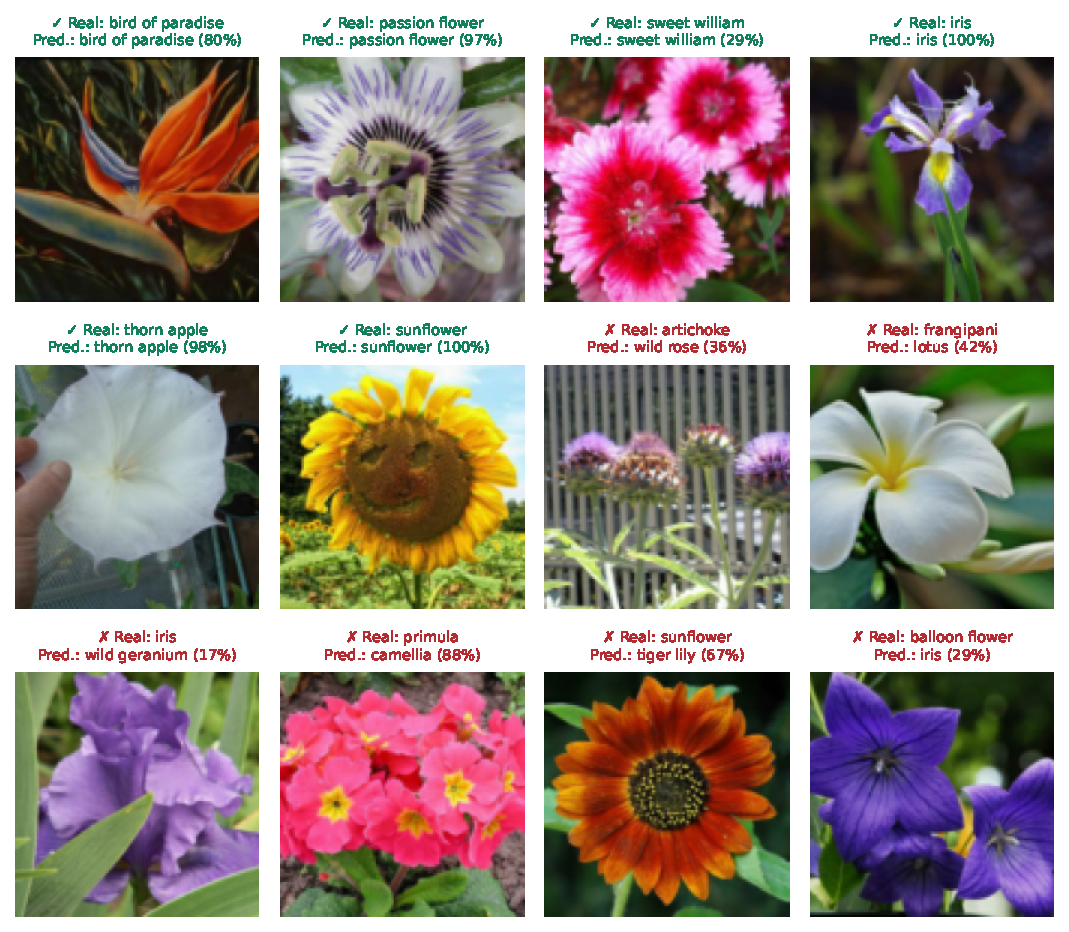
\includegraphics[width=0.8\textwidth]{predicciones_referencia.pdf}
\caption{Seis aciertos (verde, \checkmark) y seis errores (rojo, $\times$) de la
CNN de referencia en validación, elegidos con semilla fija; entre paréntesis, la
probabilidad softmax de la clase predicha. La proporción es ilustrativa: la red
acierta en 2,378 de 3,712 imágenes.}
\label{fig:predicciones}
\end{figure*}

\begin{figure}[htbp]
\centering
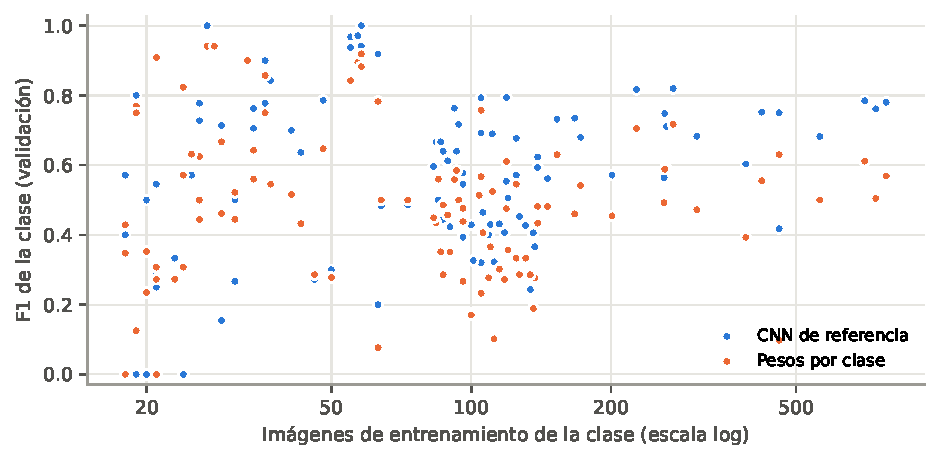
\includegraphics[width=\columnwidth]{f1_vs_tamano_clase.pdf}
\caption{F1 de validación de cada clase frente a su número de imágenes de
entrenamiento (escala logarítmica).}
\label{fig:f1-tamano}
\end{figure}

\begin{figure*}[p]
\centering
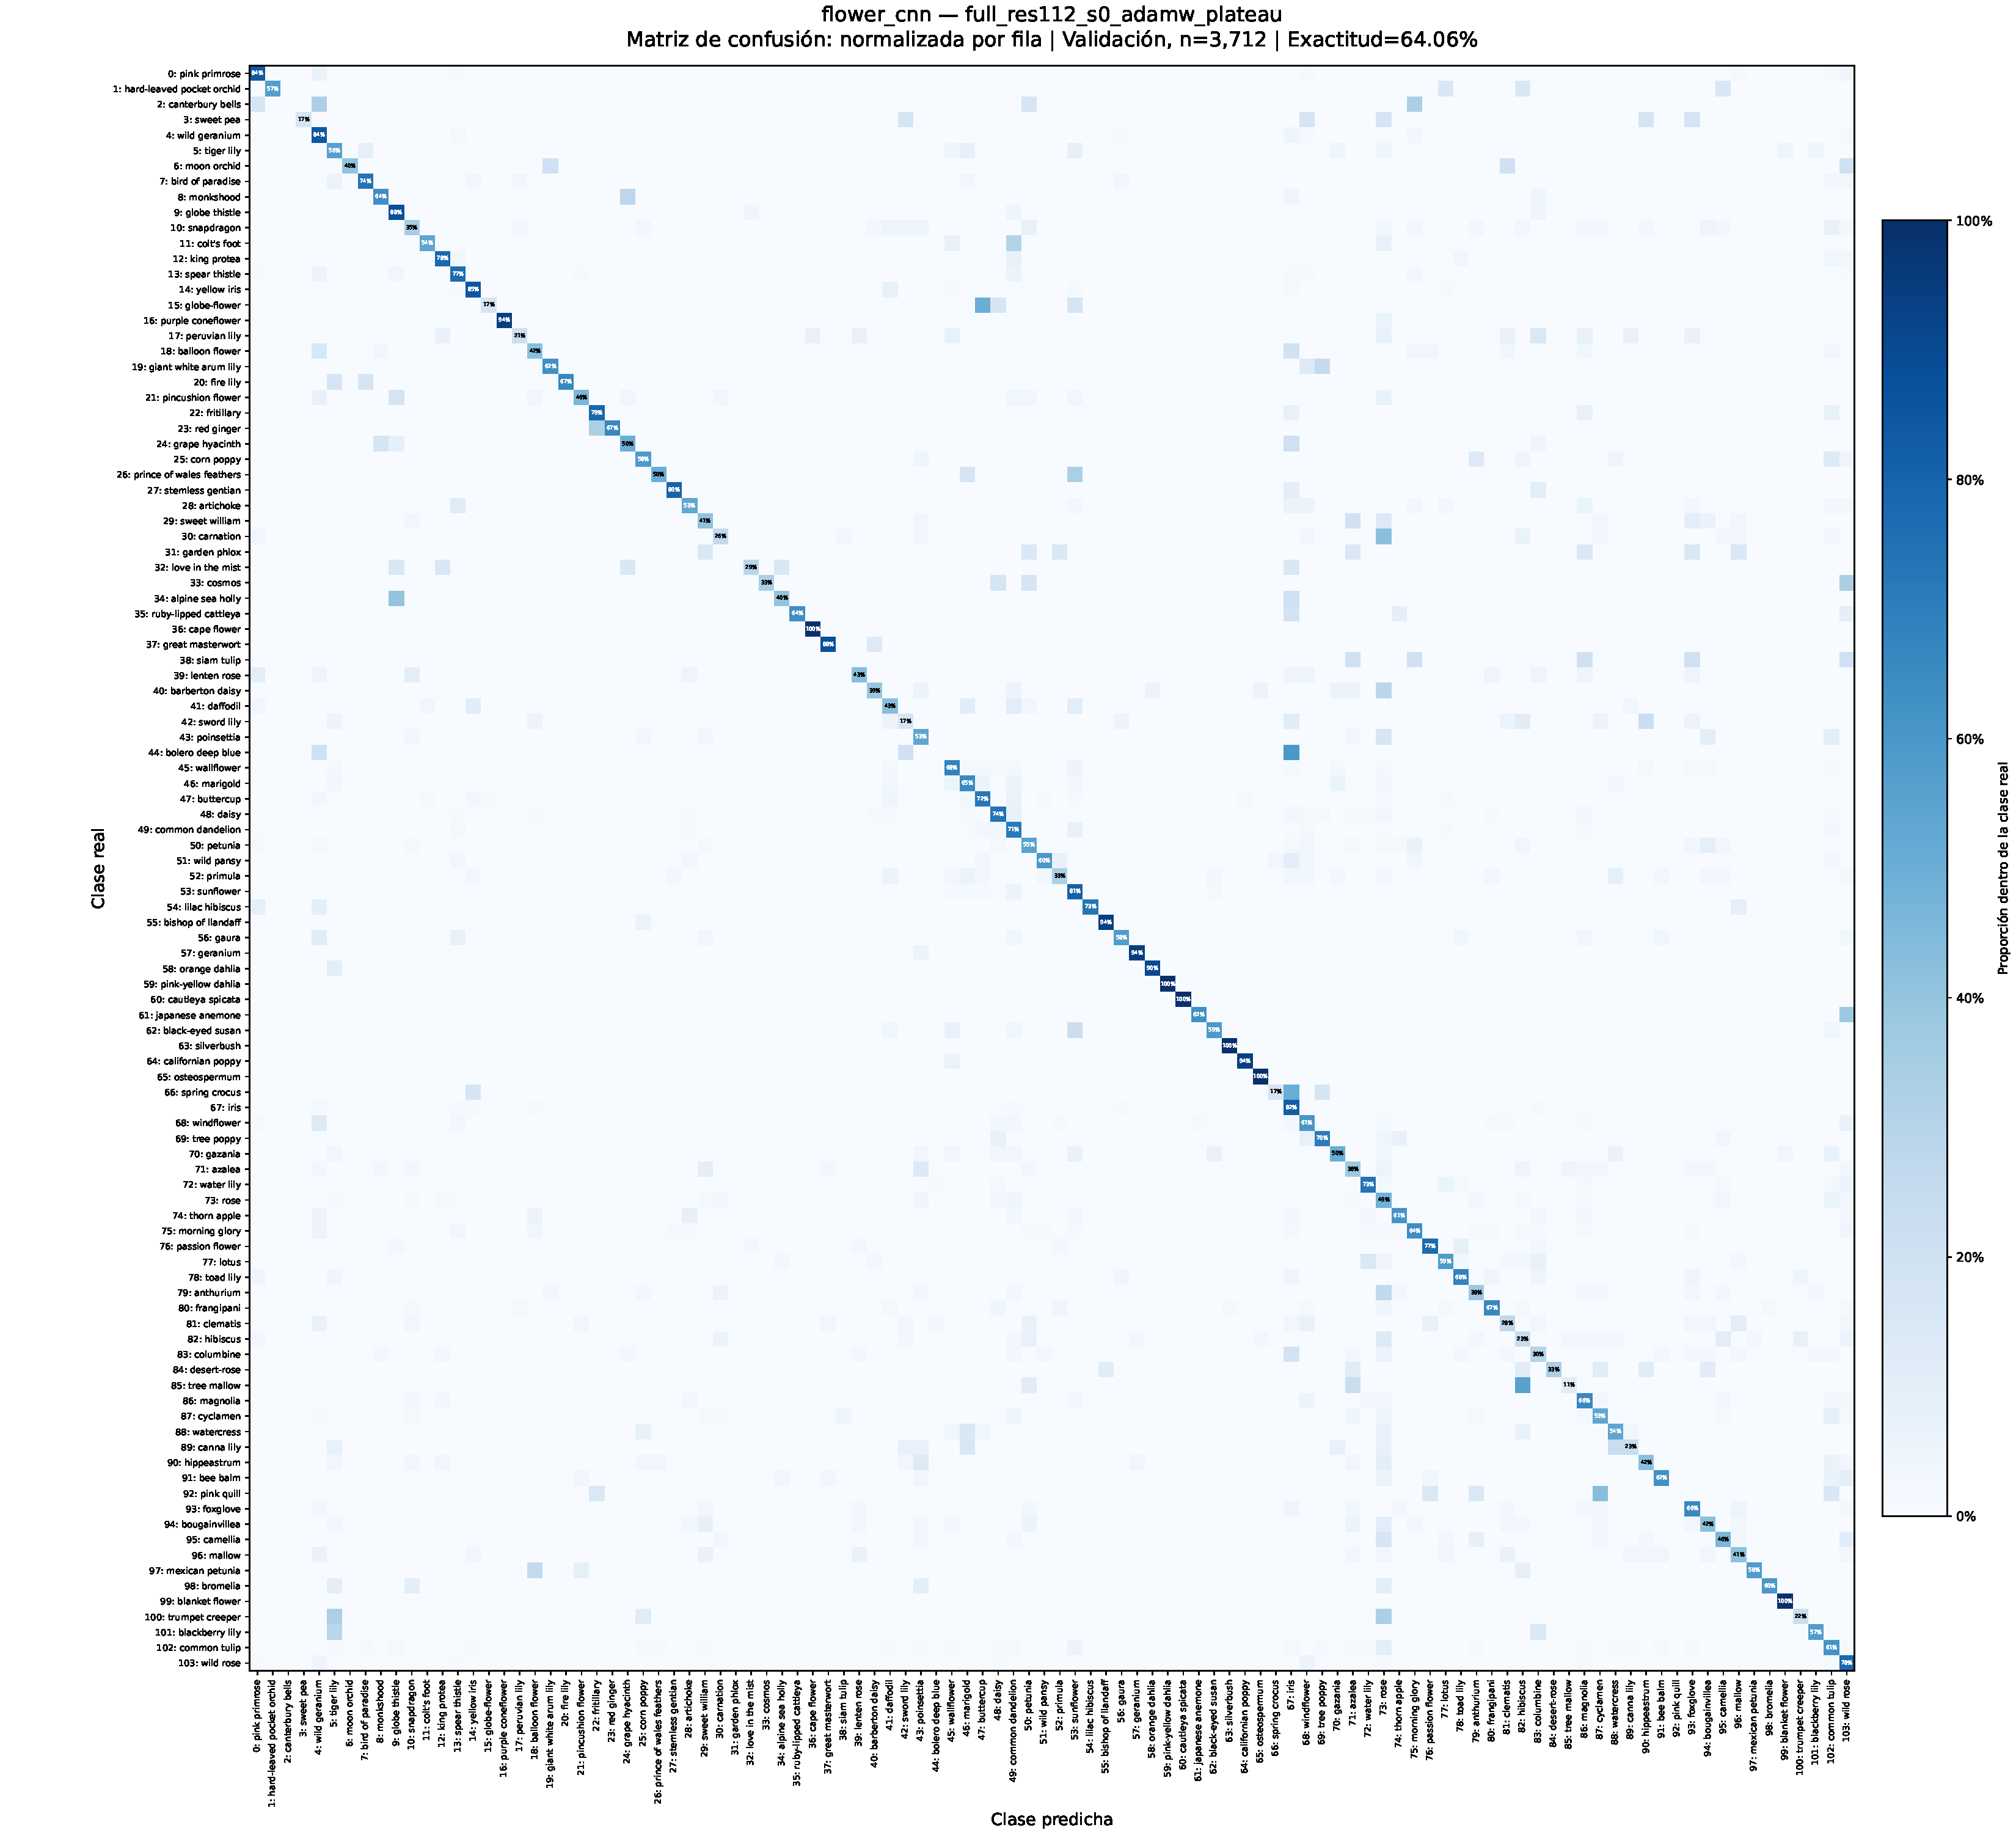
\includegraphics[width=\textwidth,height=0.85\textheight,keepaspectratio]{confusion_referencia.pdf}
\caption{Matriz de confusión normalizada por fila de la CNN de referencia en
validación (104 clases).}
\label{fig:confusion}
\end{figure*}

\subsection{Pesos por clase}
\label{sec:res-class-weight}

La variante con pesos por clase cambia solo la pérdida (Sección~\ref{sec:pesos}): misma
arquitectura, semilla, aumento, dropout y calendario de la tasa. No mejora a la
referencia (Tabla~\ref{tab:desbalance}). Su F1 macro baja de 0.5784 a 0.4881 y
su exactitud de 64.06\% a 48.87\%; 83 de las 104 clases empeoran y solo 17
mejoran.

Los pesos sí hacen lo que se espera de ellos, pero el resultado neto es
negativo. La sensibilidad (\emph{recall}) macro queda igual, 0.56 en ambas
redes, mientras que la precisión macro cae de 0.63 a 0.46: la red no reconoce
mejor las flores, solo reparte sus predicciones de otra manera. Por grupos de
tamaño se ve el intercambio:

\begin{itemize}
\item \textbf{Clases con menos de 30 imágenes (24 clases).} Su sensibilidad
sube de 0.42 a 0.61 y su F1 medio de 0.461 a 0.487. Las clases con F1 = 0
bajan de cinco a dos (\emph{bolero deep blue} y \emph{sweet pea}), y la red
llega a predecir las 104 clases (la referencia nunca predice tres). Pero las
predice de más: a las 10 clases más pequeñas les asigna 112 imágenes de
validación, cuando solo tienen 56 (la referencia les asignaba 25). Su precisión
baja de 0.58 a 0.42, y en esas 10 clases el F1 medio incluso baja un poco (de
0.361 a 0.328), aunque con 5 imágenes de validación por clase esa diferencia
está dentro del ruido.
\item \textbf{Clases con 60 o más imágenes (62 clases).} Pagan el costo. En las
nueve clases de 300 imágenes o más, la sensibilidad cae de 0.72 a 0.40 y el F1
de 0.690 a 0.481; \emph{iris}, por ejemplo, pasa de reconocer 82\% de sus
imágenes a 47\%. Las 44 clases de 60 a 149 imágenes, el grupo más grande, bajan
de 0.530 a 0.405. Como estas clases son mayoría, dominan el promedio macro.
\end{itemize}

Las confusiones cambian de dirección. En la referencia, la flor rara se
confundía con la frecuente (\emph{carnation} $\to$ \emph{rose}, 13 imágenes);
con pesos, ocurre al revés (\emph{rose} $\to$ \emph{carnation}, 15). Los pares
más confundidos son ahora \emph{wild rose} $\to$ \emph{windflower} (28),
\emph{wild geranium} $\to$ \emph{iris} (21) e \emph{iris} $\to$
\emph{wild geranium} (17). La correlación entre tamaño de clase y F1 pasa de
0.12 a $-0.06$ (Figura~\ref{fig:f1-tamano}): la dependencia del tamaño
desaparece, pero porque las clases grandes bajaron, no porque las pequeñas
subieran.

La red con pesos también aprende más despacio. En la época 40, su F1 de
validación es 0.434, contra 0.514 de la referencia, y en el checkpoint (época
70 de 82) su F1 de entrenamiento es 0.638, contra 0.814. Por eso su brecha es
menor (0.150 contra 0.235): no generaliza mejor, ajusta peor el entrenamiento.

Esta configuración se lanzó tres veces; las dos primeras corridas se
interrumpieron por bloqueos de la GPU en las épocas 64 y 68, con un mejor F1 de
0.528 y 0.531. Las tres curvas coinciden hasta la época 40 (F1 de 0.436, 0.429 y
0.434). La corrida completa, que es la que se reporta, recibió su primera
reducción de la tasa en la época 34, contra la 41--42 de las otras dos, y con
ello quedó por debajo. La GPU no es determinista aun con semilla fija, así que
una diferencia de unas 0.04 entre corridas idénticas da una idea del ruido de
una sola semilla. Con cualquiera de las tres, la conclusión es la misma: los
pesos por clase quedan entre 0.05 y 0.09 puntos de F1 por debajo de la
referencia.

\begin{table*}[htbp]
\centering
\caption{Pérdida ponderada por clase frente a la pérdida sin ponderar.}
\label{tab:desbalance}
\small
\begin{tabular}{lrrrrr}
\toprule
Entrenamiento & Exact. (\%) & F1 10 menores & F1 10 mayores & Clases F1 = 0 & F1 macro \\
\midrule
CNN de referencia & 64.06 & 0.3607 & 0.7034 & 5 & \textbf{0.5784} \\
Pesos por clase & 48.87 & 0.3281 & 0.5050 & 2 & 0.4881 \\
\bottomrule
\end{tabular}
\par\smallskip
\parbox{0.95\textwidth}{\footnotesize F1 10 menores/mayores: F1 promedio de las 10 clases con menos (18--19) y más (460--782) imágenes de entrenamiento. Pesos $w_c = N/(K\,n_c)$: van de 0.16 (iris) a 6.81 (las clases de 18 imágenes).}
\end{table*}


\subsection{Efecto de la regularización}
\label{sec:res-regularizacion}

Para medir qué aportan las técnicas de regularización, se entrenó la misma CNN,
con la misma semilla y el mismo tope de épocas, sin dropout, sin aumento de
datos y con Adam en lugar de AdamW (Tabla~\ref{tab:regularizacion} y
Figura~\ref{fig:curvas-regularizacion}). Sin regularización, la red aprende más
rápido al principio: llega a un F1 de validación de 0.5 en la época 25, frente a
la 38 de la referencia. Pero ahí se estanca. Su mejor F1 es 0.5332, 0.045 por
debajo de la referencia (0.5784), y su exactitud baja de 64.06\% a 59.64\%.

La causa es el sobreajuste. Sin regularización, el F1 de entrenamiento sube a
0.877 (0.814 con regularización) y la brecha de F1 pasa de 0.235 a 0.344. La
pérdida de validación toca su mínimo en la época 25 (1.825) y después sube hasta
2.122, mientras que con regularización su mínimo es 1.464 y prácticamente no
sube. El daño se concentra en las clases pequeñas: el F1 promedio de las 10
clases más pequeñas baja de 0.361 a 0.257, mientras que el de las 10 más grandes
solo baja de 0.703 a 0.669. Las clases con 18--30 imágenes son las más fáciles
de memorizar y, sin aumento, la red ve siempre las mismas pocas fotos.

\begin{table*}[htbp]
\centering
\caption{La misma CNN con y sin regularización (semilla 0, mismas épocas máximas).}
\label{tab:regularizacion}
\small
\begin{tabular}{lcccrrrrr}
\toprule
Variante & Dropout & Aumento & Pesos & Época & Exact. (\%) & F1 entr. & Brecha F1 & F1 macro \\
\midrule
CNN de referencia & 0.5 & sí & WD 0.01 & 91/103 & 64.06 & 0.8138 & +0.2354 & \textbf{0.5784} \\
Sin regularización & 0 & no & -- & 34/46 & 59.64 & 0.8767 & +0.3435 & 0.5332 \\
\bottomrule
\end{tabular}
\par\smallskip
\parbox{0.95\textwidth}{\footnotesize Pesos: WD = weight decay desacoplado de AdamW; -- = Adam sin decaimiento. Ambas comparten arquitectura, tasa de aprendizaje inicial, reducción de LR en meseta, paciencia de 12 evaluaciones y tope de 150 épocas.}
\end{table*}


\begin{figure*}[htbp]
\centering
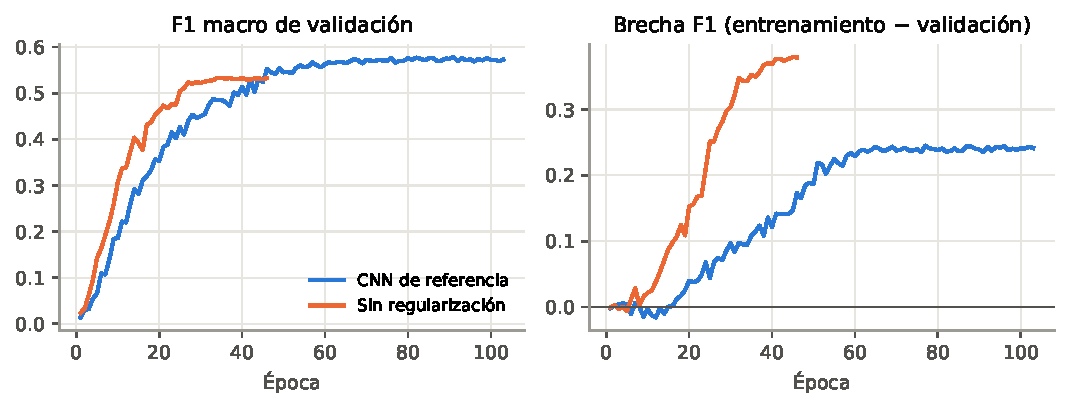
\includegraphics[width=0.85\textwidth]{curvas_regularizacion.pdf}
\caption{F1 macro de validación y brecha de F1 por época, con y sin
regularización (misma semilla, arquitectura y tope de épocas).}
\label{fig:curvas-regularizacion}
\end{figure*}

\subsection{Hiperparámetros}
\label{sec:res-hiperparametros}

La Tabla~\ref{tab:hiperparametros} cambia un hiperparámetro a la vez respecto
a la referencia, con el conjunto completo de entrenamiento. Ninguna de las dos
variantes la mejora:

\begin{itemize}
\item \textbf{Tasa de aprendizaje de $3\times10^{-4}$ (en vez de
$10^{-3}$): F1 0.4605.} Es la peor de las CNN, pero no por sobreajuste: su brecha
de F1 es solo 0.094 porque la red tampoco aprende bien el entrenamiento (F1 de
entrenamiento 0.554, contra 0.814 de la referencia). La reducción automática de
la tasa ocurre cuando la pérdida de validación deja de mejorar dos épocas; al
partir de una tasa ya baja, en pocas reducciones llega al mínimo de $10^{-5}$ y
el aprendizaje prácticamente se detiene. En la época del checkpoint (98) la tasa
ya estaba en ese mínimo. Es infraajuste causado por el calendario de la tasa, no
por la capacidad de la red.
\item \textbf{Dropout de 0.3 (en vez de 0.5): F1 0.5596.} Con menos dropout,
el F1 de entrenamiento es prácticamente igual (0.816 contra 0.814), pero el de
validación baja 0.019 y la brecha sube de 0.235 a 0.256. Es el mismo patrón que
sin regularización, en menor grado: menos regularización, más memorización. De
nuevo, las clases pequeñas son las que más pierden (0.286 contra 0.361).
\end{itemize}

Con una sola semilla, la diferencia de 0.019 del dropout es moderada; la de la
tasa de aprendizaje (0.118) es clara.

\begin{table*}[htbp]
\centering
\caption{Efecto de un hiperparámetro a la vez, con el conjunto completo.}
\label{tab:hiperparametros}
\small
\begin{tabular}{lcccrrrrr}
\toprule
Configuración & LR & Dropout & Resolución & Época & Exact. (\%) & Brecha F1 & Tiempo (min) & F1 macro \\
\midrule
CNN de referencia & 0.001 & 0.5 & 112 & 91/103 & 64.06 & +0.2354 & 19.7 & \textbf{0.5784} \\
LR $3\times10^{-4}$ & 0.0003 & 0.5 & 112 & 98/110 & 54.18 & +0.0936 & 22.5 & 0.4605 \\
Dropout 0.3 & 0.001 & 0.3 & 112 & 61/73 & 61.96 & +0.2561 & 15.0 & 0.5596 \\
\bottomrule
\end{tabular}
\par\smallskip
\parbox{0.95\textwidth}{\footnotesize Cada fila cambia un solo valor respecto a la referencia (LR $10^{-3}$, dropout 0.5, 112$\times$112).}
\end{table*}


\subsection{Reducción de datos con Distribution Matching}
\label{sec:res-dm}

Como experimento independiente de los anteriores, se evaluó si un conjunto
pequeño de imágenes sintéticas generado con Distribution Matching (DM)
\autocite{zhao2023dm} conserva
más información que el mismo número de imágenes reales elegidas al azar
(Tabla~\ref{tab:dm}). Con una imagen por clase (IPC 1, 104 imágenes), DM supera
a la selección aleatoria (F1 0.067 frente a 0.051). Con diez por clase
(IPC 10, 1,040 imágenes) ocurre lo contrario: las imágenes reales dan 0.258 y
las sintéticas 0.204, con más variación entre semillas. La destilación ayuda
solo cuando hay muy pocas imágenes, y su costo (16 y 25 minutos de generación)
se suma al del entrenamiento. Ninguna de estas imágenes se usó en los demás
experimentos; todos entrenan con las 12,753 imágenes reales.

\begin{table}[htbp]
\centering
\caption{Selección aleatoria frente a destilación con Distribution Matching (DM).}
\label{tab:dm}
\small
\begin{tabular}{rrlrrr}
\toprule
IPC & Imágenes & Conjunto & Exact. (\%) & F1 macro & Destilación (min) \\
\midrule
1 & 104 & Sintéticas (DM) & 9.85 & 0.0672 $\pm$ 0.0052 & 16 \\
1 & 104 & Reales aleatorias & 5.75 & 0.0514 $\pm$ 0.0029 & -- \\
10 & 1,040 & Sintéticas (DM) & 20.55 & 0.2044 $\pm$ 0.0235 & 25 \\
10 & 1,040 & Reales aleatorias & 25.86 & 0.2575 $\pm$ 0.0082 & -- \\
\bottomrule
\end{tabular}
\par\smallskip
\parbox{0.95\textwidth}{\footnotesize Promedio $\pm$ desviación estándar de tres semillas de entrenamiento por condición. Misma CNN, Adam $10^{-3}$, $112\times112$. Datos: \path{reports/resultados.csv}.}
\end{table}


